% \begin{figure*}[!ht]
%     \centering
%     \subfloat[gas]{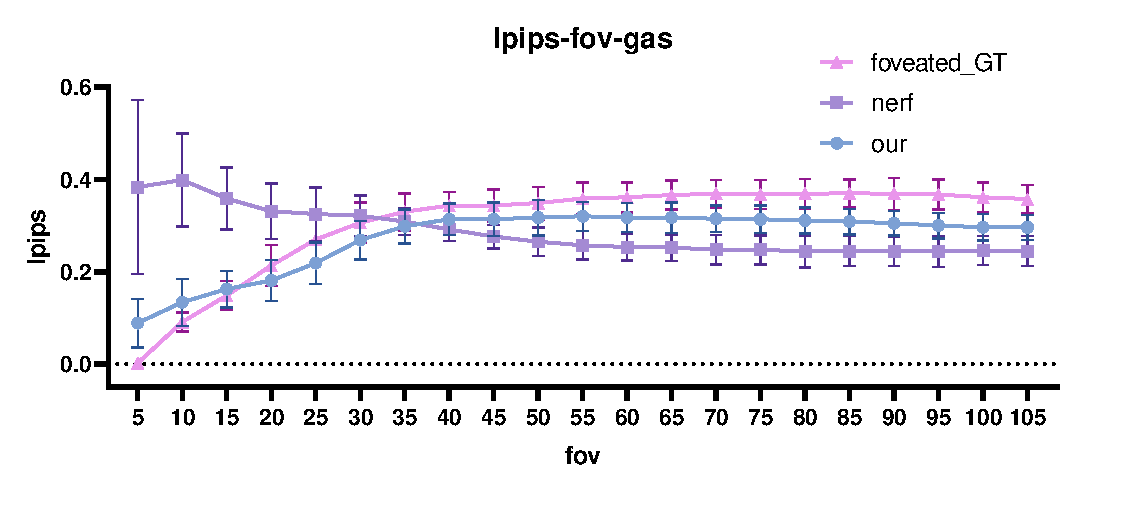
\includegraphics[width=0.48\linewidth]{TOG/figs/lpips-fov-gas-group.pdf}}\label{lpips:gas}
%     \subfloat[minecraft]{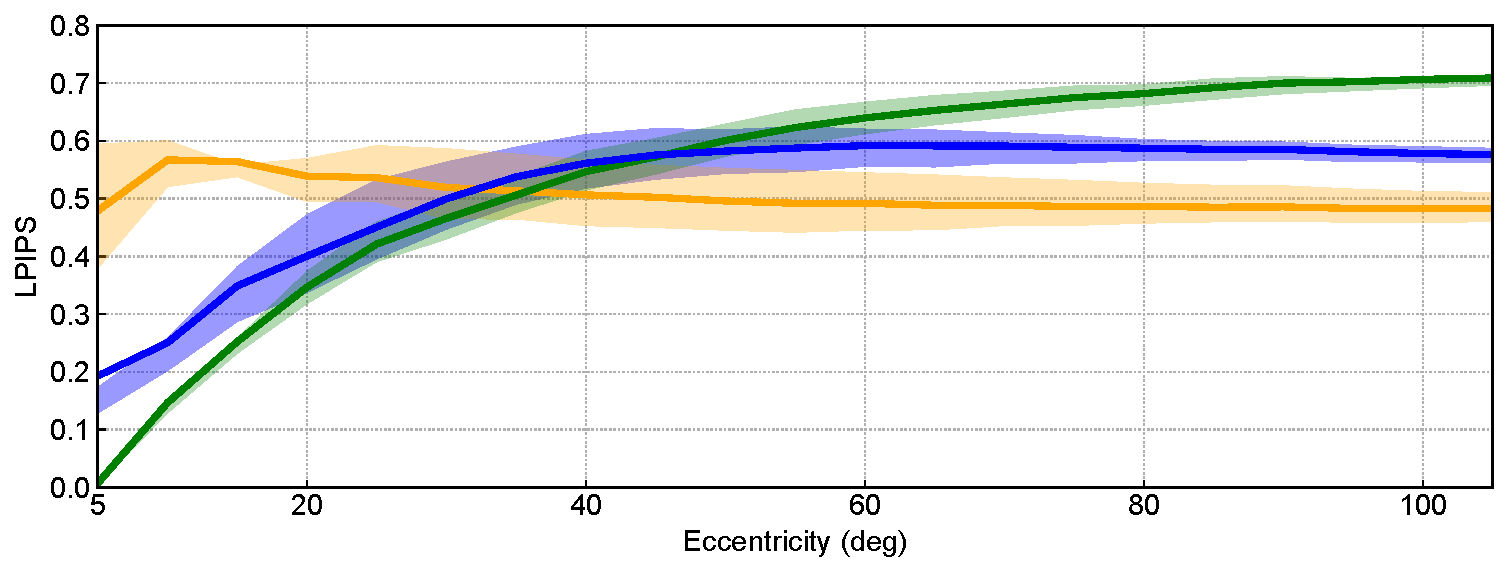
\includegraphics[width=0.48\linewidth]{TOG/figs/lpips_scenemc.pdf}}
    
%     \subfloat[studyroom]{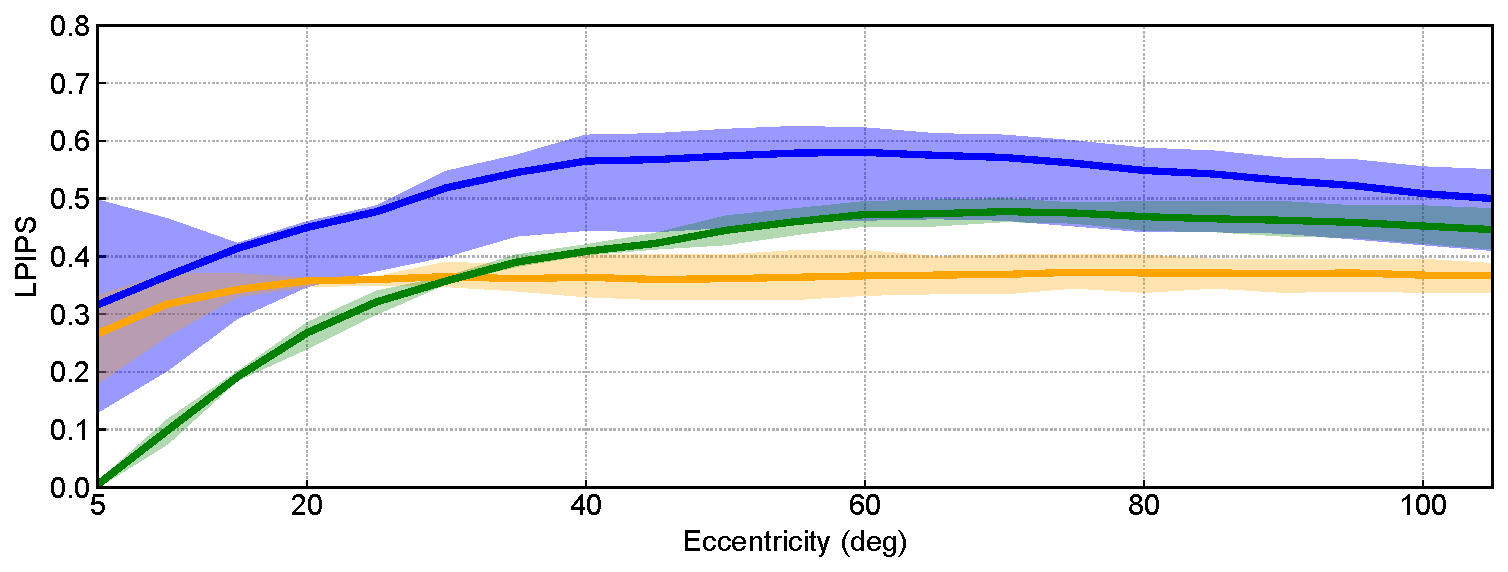
\includegraphics[width=0.48\linewidth]{TOG/figs/lpips_scenestudyroom.pdf}}
%     \subfloat[bedroom]{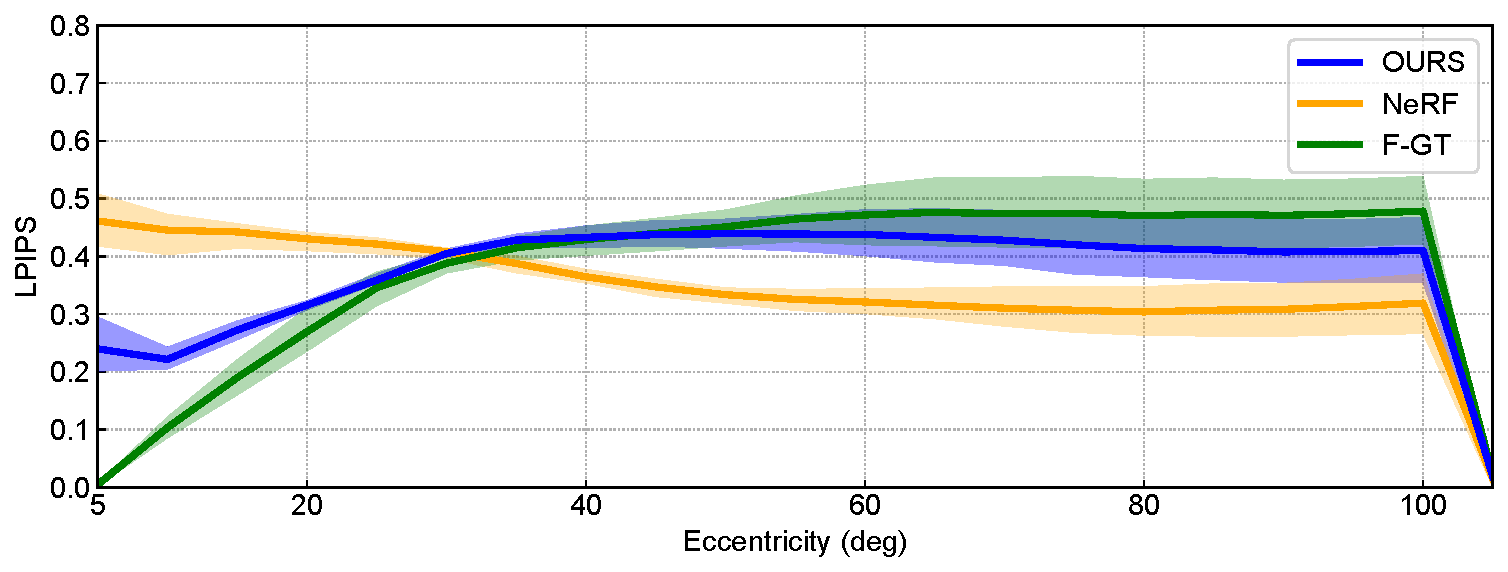
\includegraphics[width=0.48\linewidth]{TOG/figs/lpips_scenebedroom.pdf}}
%     \caption{LPIPS analysis of four scenes as well as comparison of our method, NeRF, and foveated GT on each eccentricity.}
%     {We found a significant difference in \warning{ecc range} between \warning{stimulus} and \warning{stimulus};}
%     \label{fig:lpips}
% \end{figure*}

% ZH: why \Cref{fig:lpips:gas} shows 'section 5.2'
\begin{figure*}[ht]
    \centering
    \subfloat[gas]{\label{fig:lpips:gas}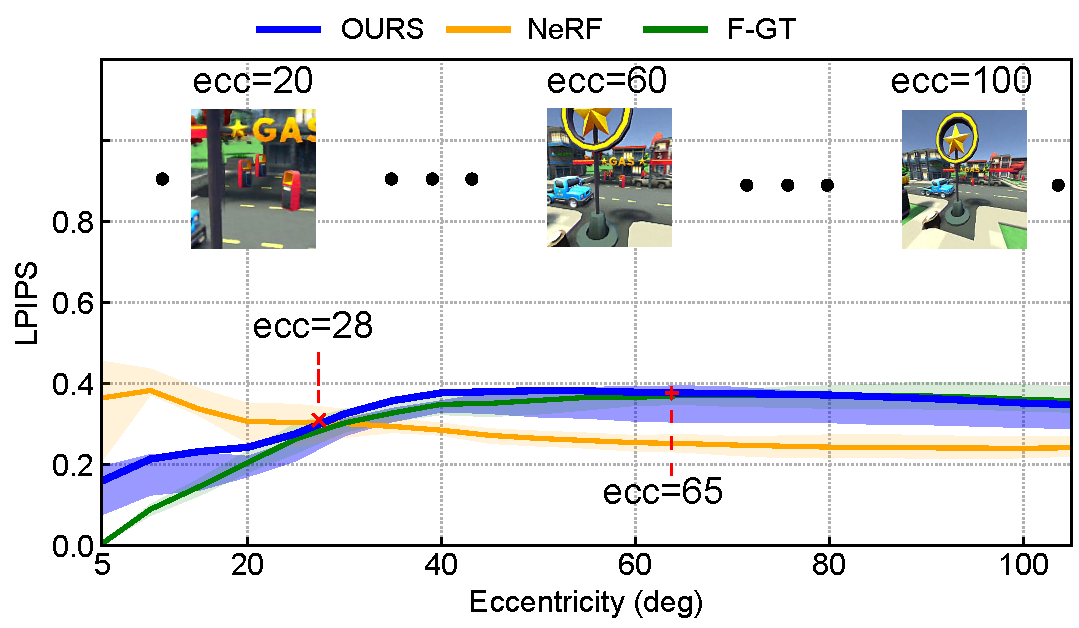
\includegraphics[width=0.48\linewidth]{TOG/figs/lpips/lpips-gas-84.pdf}}
    \subfloat[minecraft]{\label{fig:lpips:mc}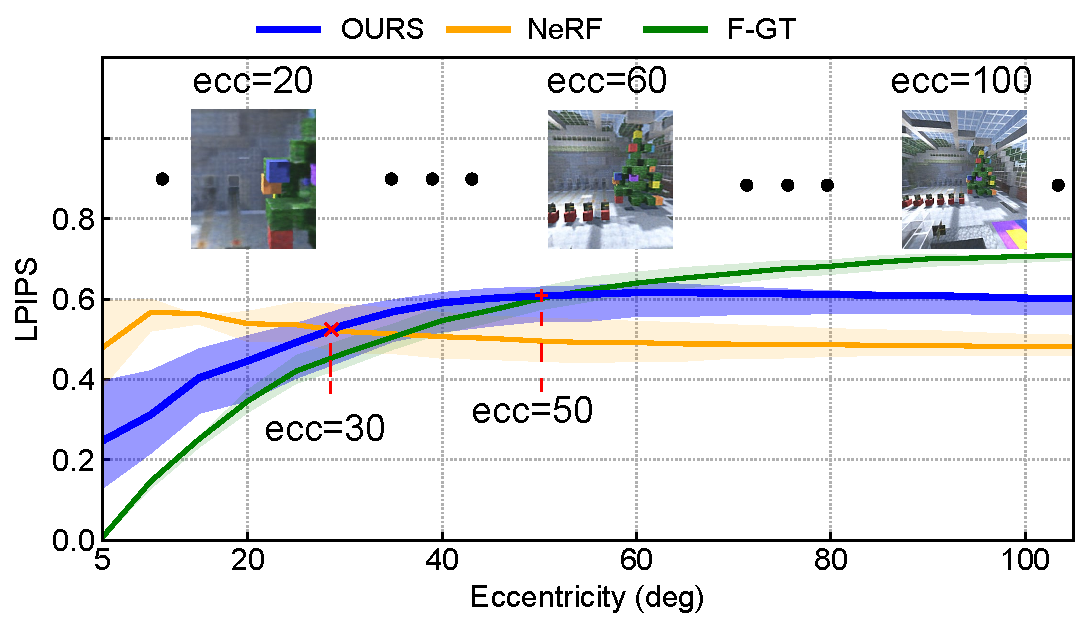
\includegraphics[width=0.48\linewidth]{TOG/figs/lpips/lpips-mc-84.pdf}}
    
    \subfloat[gallery]{\label{fig:lpips:gallery}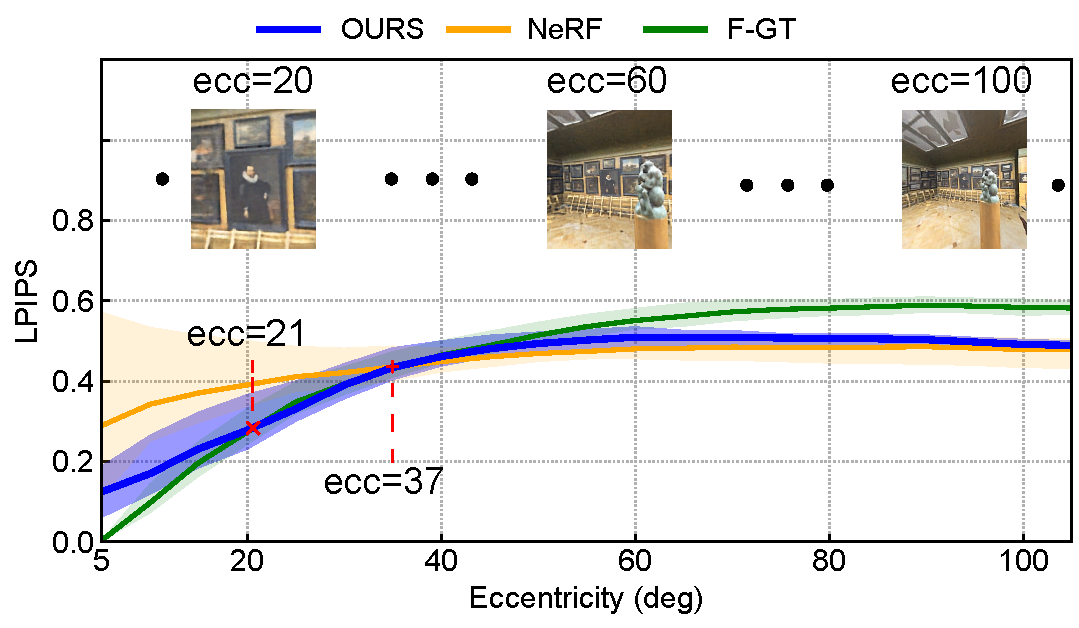
\includegraphics[width=0.48\linewidth]{TOG/figs/lpips/lpips-gallery-84.pdf}}
    \subfloat[bedroom]{\label{fig:lpips:bedroom}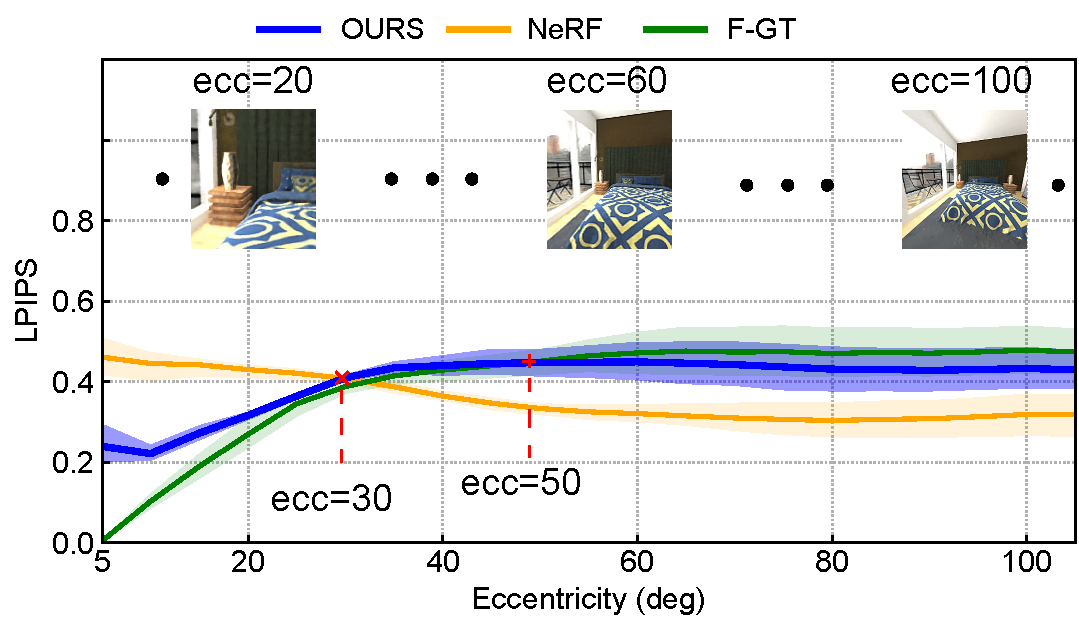
\includegraphics[width=0.48\linewidth]{TOG/figs/lpips/lpips-bedroom-84.pdf}}
    \Caption{LPIPS visualization of all scenes as well as comparison of {\bf OURS}, {\bf NeRF}, and {\bf F-GT} over the visual field.}
    {%
    X-axis indicate eccentricity range ($0$ to 110). Y-axis shows the LPIPS loss \cite{zhang2018unreasonable} with a full resolution rendering as reference. Lower values mean more similar perceptual quality to the reference. The semi-transparent layer indicate first and third quarterlies. The inset figures' corresponding eccentricity ranges are indicated by the dashed lines.
    }
    \label{fig:lpips}
\end{figure*}